\documentclass[final]{siamltexmm}
\documentclass[10pt,a4paper]{article}

\usepackage{graphicx}
\usepackage{algorithm}
\usepackage{algorithmic}

% \usepackage[demo]{graphicx}
% \usepackage{subfig}

\newcommand{\pe}{\psi}
\def\d{\delta} 
\def\ds{\displaystyle} 
\def\e{{\epsilon}} 
\def\eb{\bar{\eta}}  
\def\enorm#1{\|#1\|_2} 
\def\Fp{F^\prime}  
\def\fishpack{{FISHPACK}} 
\def\fortran{{FORTRAN}} 
\def\gmres{{GMRES}} 
\def\gmresm{{\rm GMRES($m$)}} 
\def\Kc{{\cal K}} 
\def\norm#1{\|#1\|} 
\def\wb{{\bar w}} 
\def\zb{{\bar z}} 

% some definitions of bold math italics to make typing easier.
% They are used in the corollary.

\def\bfE{\mbox{\boldmath$E$}}
\def\bfG{\mbox{\boldmath$G$}}

\title{Deep Learning Assignment 2}
\author{Yun-shao Sung\thanks{\tt yss265@nyu.edu}
        \and Chung-Ling Yao\thanks{\tt cly264@nyu.edu}}

\begin{document}
\maketitle

\begin{abstract}
This is the report for deep learning assignment 2
\end{abstract}

\pagestyle{myheadings}
\thispagestyle{plain}

\section{More Backpropagation}
\subsection{Backpropagation through a DAG of modules}
Given each node is sigmoid layers, and the second layer is $O_{min} = min(i_{1}, i_{2})$ and $O_{max} = max(i_{1}, i_{2})$. Therefore, we can rewrite $y$ as:
\begin{equation}
y = min({1\over1+e^{-x_{1}}}, {1\over1+e^{-x_{2}}}) + max({1\over1+e^{-x_{1}}}, {1\over1+e^{-x_{2}}})
\end{equation}
which can also rewrite as:
\begin{equation}
y = {1\over1+e^{-x_{1}}} + {1\over1+e^{-x_{2}}}
\end{equation}
as we taking the deritive of $E$ respect to $x_{i}$ and with chain rule applied:
\begin{equation}
{\partial E\over \partial x_{i}} = {\partial E\over \partial y} {e^{-x_{i}} \over (1+e^{x_{i}})^2}}
\end{equation}

\subsection{Batch Normalization}
\subsubsection{Calculate {\partial E\over \partial x_k}}
Let us concentrate on a particular activation $x_k$, which is a mini-batch $\beta$ of size m
\begin{equation}
\beta=\{{x_{1...m}}\}
\end{equation}
mean of this mini-batch:
\begin{equation}
\mu_\beta={1\over m} \sum\limits_{i=1}^{m}x_i
\end{equation}
variance of this mini-batch:
\begin{equation}
\sigma^2_\beta={1\over m} \sum\limits_{i=1}^{m}(x_i-\mu_\beta)^2
\end{equation}
By definition:
\begin{equation}
y_i={{x_i-\mu_\beta}\over \sqrt{\sigma^2_\beta}} 
\end{equation}

Since $\sigma^2_\beta$ and $\mu_\beta$ are function of $x_i$, we have to calculate ${\partial E \over \partial \sigma^2_\beta}$ and ${\partial E \over \partial \mu_\beta}$
\begin{equation}
{\partial E \over \partial \sigma^2_\beta}=\sum\limits_{i=1}^{m} {\partial E \over \partial y_i}\cdot {\partial y_i \over \partial \sigma^2_\beta} 
=\sum\limits_{i=1}^{m} {\partial E \over \partial y_i}\cdot (x_i-\mu_\beta) \cdot {-1 \over 2} (\sigma^2_\beta)^{3 \over 2}
\end{equation}

\begin{equation}
{\partial E \over \partial \mu_\beta}=
\sum\limits_{i=1}^{m} {\partial E \over \partial y_i}\cdot {\partial y_i \over \partial \mu_\beta} + {\partial E \over \partial \sigma^2_\beta} \cdot {\partial \sigma^2_\beta \over \partial \mu_\beta}
=(\sum\limits_{i=1}^{m} {\partial E \over \partial y_i}\cdot {-1 \over {\sqrt{\sigma^2_\beta}}})+ {\partial E \over \partial \sigma^2_\beta} \cdot {{\sum\limits_{i=1}^{m}{-2(x_i-\mu_\beta)}} \over {m}}
\end{equation}

\begin{equation}
{\partial E\over \partial x_i}={\partial E\over \partial y_i} {\partial y_i\over \partial x_i}+{\partial E\over \partial \sigma^2_\beta} {\partial \sigma^2_\beta \over \partial x_i}+{\partial E\over \partial \mu_\beta} {\partial \mu_\beta\over \partial x_i}
={\partial E\over \partial y_i} \cdot {1 \over {\sqrt{\sigma^2_\beta}}}+{\partial E\over \partial \sigma^2_\beta} \cdot {2(x_i-\mu_\beta) \over {m}}+{\partial E\over \partial \mu_\beta}\cdot{1 \over m}
\end{equation}

\subsubsection{Shift variable}
Let $\varepsilon$ be a learnable shift variable, we can define the formula as:\\
forward pass:
\begin{equation}
y_k={x_k-E(x_k)\over {\sigma(x_k)}}+\varepsilon_k
\end{equation}

backward pass:
\begin{equation}
{\partial E\over \partial x_i}={\partial E\over \partial y_i} {\partial y_i\over \partial x_i}+{\partial E\over \partial \sigma^2_\beta} {\partial \sigma^2_\beta \over \partial x_i}+{\partial E\over \partial \mu_\beta} {\partial \mu_\beta\over \partial x_i}
={\partial E\over \partial y_i} \cdot {1 \over {\sqrt{\sigma^2_\beta}}}+{\partial E\over \partial \sigma^2_\beta} \cdot {2(x_i-\mu_\beta) \over {m}}+{\partial E\over \partial \mu_\beta}\cdot{1 \over m}
\end{equation}


\begin{equation}
{\partial E\over \partial \varepsilon}
=\sum\limits_{i=1}^{m}{\partial E\over \partial y_i}\cdot{\partial y_i\over \partial \varepsilon}
=\sum\limits_{i=1}^{m}{\partial E\over \partial y_i}\cdot{\partial \over \partial \varepsilon}{( {x_i-E(x_k)\over {\sigma(x_k)}}+\varepsilon_k )}
=\sum\limits_{i=1}^{m}{\partial E\over \partial y_i}
\end{equation}

\\
\section{STL-10: semi-supervised image recognition}
\subsection{Method: Surrogate Class}
We were trying to create surrogate training data from unlabeled images. As the reference paper mentioned, we ramdonly choose 4000 unlabel images and obtain patches from different images at varying positions and scales. The tansformation $\{T_{\alpha}|\alpha \in A\}$ parameterized by vectors $\alpha$ and $A$ is a set of random possible tranformation. Therefore, each tranformation $T_{\alpha}$ is a combination of each transformation below:\\\\

1. Rotation with random degree in range $[-10, 10]$\\
2. Translate random horizontally and vertically in range $[0, 0.1]$ of patch size\\
3. Scale with random degree in range $[1, 1.4]$ of patch size\\
4. Randomly decide to perform hflip\\\\
The procedures mentioned above are applied to unlabel images after normalization. Figure 3.1 showes the example surrogate figures. According to the reference paper, they constructed the convolution neuron network for either 64c-64c-128 or 64c5-128c5-256c5-512f, which letter $c$ represent number of convolutional filters and $f$ represent the number of fully connected units. As we randomly selected 4000 unlabel images and create 100 surrogate set per image, we got total 400000 patches which belongs to 4000 class. The techinical difficulity for this method is the time complexity because the reference paper took 4 days to train the second model, and when we did face the issue when contruct and train the model. Therefore, we realized this model may not suitable for this assignment and decided to move to other model.

\subsection{Method: K­means Centroids}
We implemented Kmeans methods as one of our model, since based on previous paper that they can reach very good performance based on this simple model. The idea can divided into two part: first for getting centroids, and the second is perform feature mapping and perform classification. Regarding to the centroids identification, we did the following three steps: \\\\
1. Randomly select certain amount of unlabeled training images, and extract random patches. The size of patch is 22x22\\
2. Apply pre-processing to patches, including normalization and whitening\\
3. Learn feature-mapping using unsupervised method, and here we use kmeans due to the its good performance in the reference paper\\\\
After centroids are identified, the steps for the second stage is as followed:\\
1. Extract patches from input images. The size of patches is 22x22, and the gap between patches is 2, and therefore we can get 16 patches from each of imput figure. Then we perforem feature mapping as the following equation:
\begin{equation}
{f_{k}(x) = max\{0, \mu(z)-z_{k}\}}
\end{equation}
where $\[ z_{k} = \norm{x-c^{(k)}} \]$ and $\mu(z)$ is the mean of the elements of $z$\\
2. Pool features together over region and perform 4 quadrants summation to reduce the number of feature values, and therefore we will get the feature in the size of $4k$ per figure, and $k$ is the number of centroids.\\
3. Perform classification based on the feature vector, and here we used 1-vs-N SVM.\\
Figure 3.2 demonstrate the procedures mentioned above, and also shows the example of centroids during the processes. As we can see from Table 2.1, when the number of 1600 centroids is fixed and changing the number of 1-vs-N SVM iterations, the accuracy is improving but not good enough. We are thinking there are few points need to take care more delicatly, for example the way of normalization, whitening, and 4 quadrants for dimension reduction.
\begin{table}[H]
\begin{center}
    \begin{tabular}{| c | c | c |}
    \hline
    numIter & Training Accuracy (\%) & Test Accuracy (\%) \\ \hline
    500 & 20.3 & 16.1 \\ \hline
    1000 & 22.4 & 18.1 \\ \hline
    10000 & 26.2 & 18.5 \\ \hline
    \end{tabular}
\end{center}
\caption{The training and test accuracy of kmeans implementation based on reference paper}
\end{table}

\subsection{Method: VGG+Kmeans+Surrogate}
Here we decide not to following the exact methoded mentioned in the reference papers, but to combine their high level ideas together. For example, the idea of kmeans is to find the centroids which will be a good representive for the small patches. Also, the idea of surrogate is to increase the size of training set by randomly transformation and therefore may give training model more different angles to learn the figure and better to predict the unlabel figures. For the left figure at figure 2.1, as we initially running the original vgg model, the training set is keep improving but not validation set after epoch 50. This suggests the training set may found a point that is good to optimize toward it but seems it's just a local minimum as we can see it not able to improve the validation set. \\
As the training process is pretty much all about updating the appropriate weighting, we think assigning a proper initial weighting will help the optimization away from local but more toward global minimum. Therefore, as centroids from the kmeans method is a good representation of patches, we decide to assign the centroids to the weighting of the first convolution layer in vgg model. The first layer performs SpatialConvolution from 3 input plane to 64 output plane with 3x3 patch size, and therefore the weighting of this layer is in the size of 64x3x3x3. To match the size of this layer, we used almost the same method mentioned above, but to randomly select 10 patches of size 3x3 from each of label figures, and run kmeans for 64 centroids. After those 64 centroids are found, we assigned the value to the first SpatialConvolution layer before the training. As we can see from the second figure in figure 2.1, generally the value for the validation set is lifting up from 68\% in original vgg model to 72\%.\\
However, we can still see the phenomenon that the training set keep improving but not the validation set, and we think the kmeans initialization indeed gave it a good start to train, but now the limitation is still the size of training set cannot reflect to the unlabel data to give the proper prediction. Therefore, we dicide to create 10 surrogate figrues with the transformation mentioned above from each of the 4000 label figures, and therefore now we get 44000 training set with the original figure and surrogate figure included. The training curve become very interesting. First of all we can see the prediction for validation set sometimes even outperform the training set, and also we can see the prediction gep between training and validation set are much close then the other models. However, limitation can still observed after epoch 50 that training still improving but not the validation set, suggesting surrogate indeed provide improvement but addition new figures may still required for model to learn from something new and potentially will need to include the method of Pseudo­labels.
\begin{table}[H]
\begin{center}
    \begin{tabular}{| c | c | c |}
    \hline
    Method & Best Validation Accuracy (\%) \\ \hline
    vgg & 68.6 \\ \hline
    vgg+kmeans & 73.7 \\ \hline
    vgg+kmeans+surrogate & 76.9 \\ \hline
    \end{tabular}
\end{center}
\caption{Accuracy of different model}
\end{table}

\begin{figure}[H]
\centering
\begin{subfigure}
  \begin{tabular}{cccc}
  \subfloat{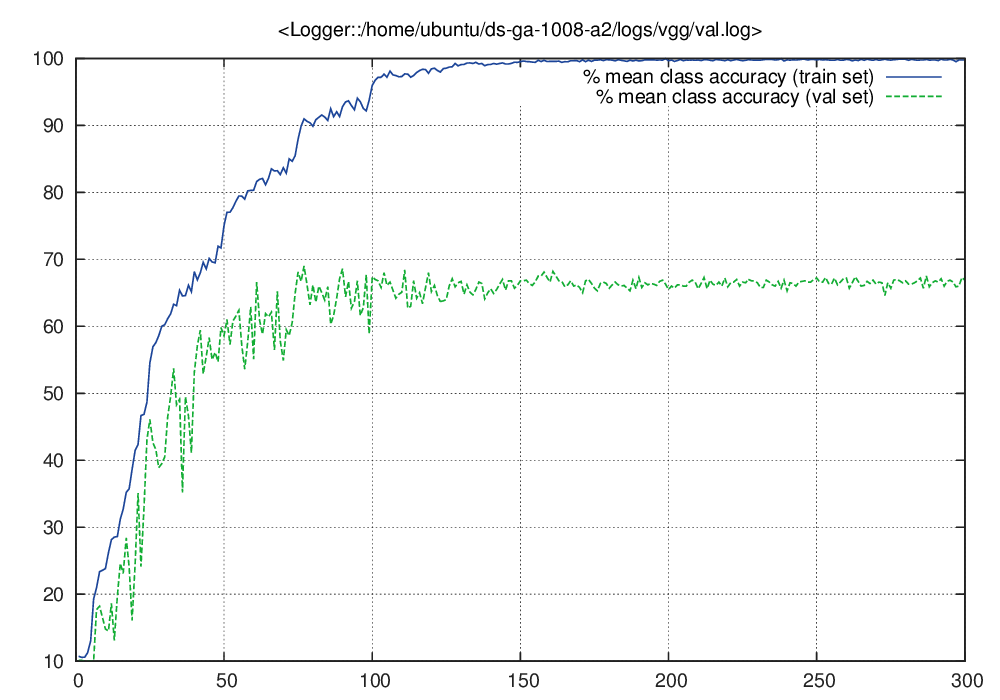
\includegraphics[width = 50mm]{../fig/models/vgg.png}}&
  \subfloat{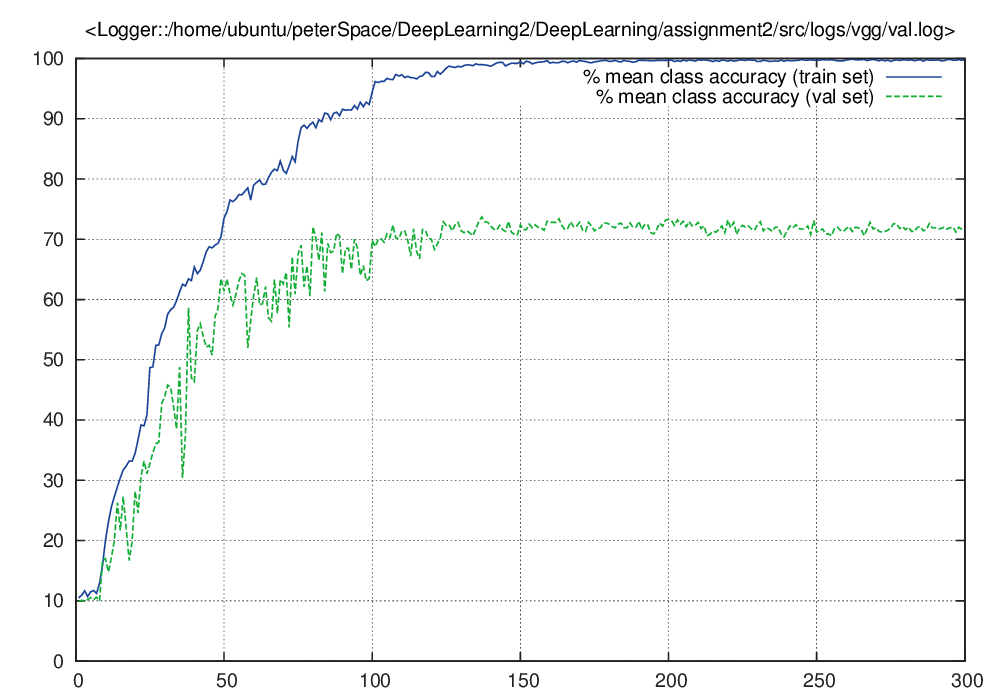
\includegraphics[width = 50mm]{../fig/models/vgg_kmeans.png}}&
  \subfloat{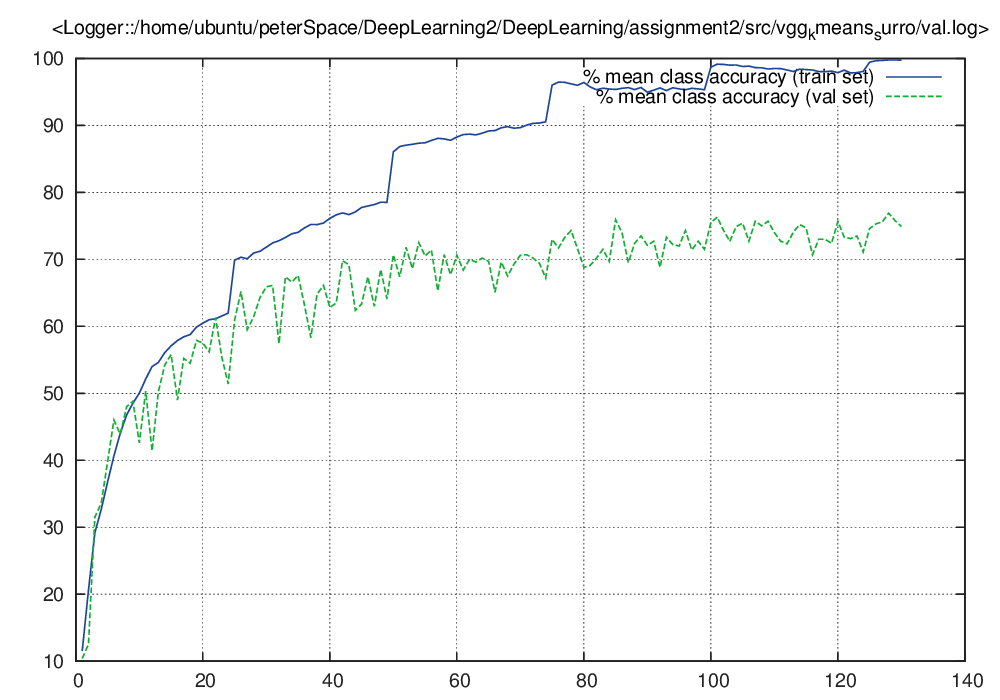
\includegraphics[width = 50mm]{../fig/models/vgg_kmeans_surro.png}}&
  \end{tabular}
\end{subfigure}
\caption{Training curve for original vgg, vgg+kmenas, and vgg+kmeans+surrogate}
\end{figure}

\subsection{Method: Pseudo­labels}
We started with the trained baseline model. For every 5 epochs, use the current model to predict 1000 unlabeled figures. We collected 100 figures out of 1000 having largest confidence (the largest prediction probabilities) and used the predicted classes as the real labels of these figures. Then we merged these new "labeled" figures into the training set and used them to train the model. We started with 4000 training set and terminated at 8800 training set. The training process was interrupted by "Out of Memory" for several times, so the training result is splited into several pictures. From the training result, we found this method didin't help to improve the validation accuracy. 
\begin{figure}[H]
\centering
\includegraphics[width=100mm]{../fig/Pseudo­labels.png}
  \caption{Pseudo­labels model}
\end{figure}

\begin{figure}[H]
\centering
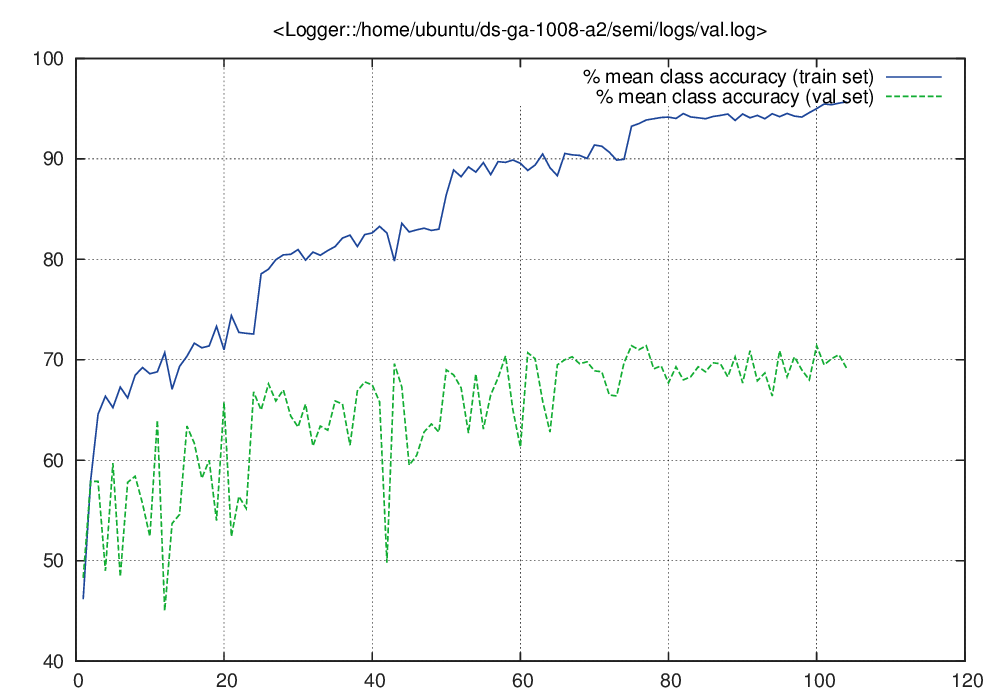
\includegraphics[width = 140mm, height=90mm]{../fig/pseudo_label/val_7100.png}
  \caption{Pseudo­labels training result: training set start from 5000 figures and end at 7100.}
\end{figure}

\begin{figure}[H]
\centering
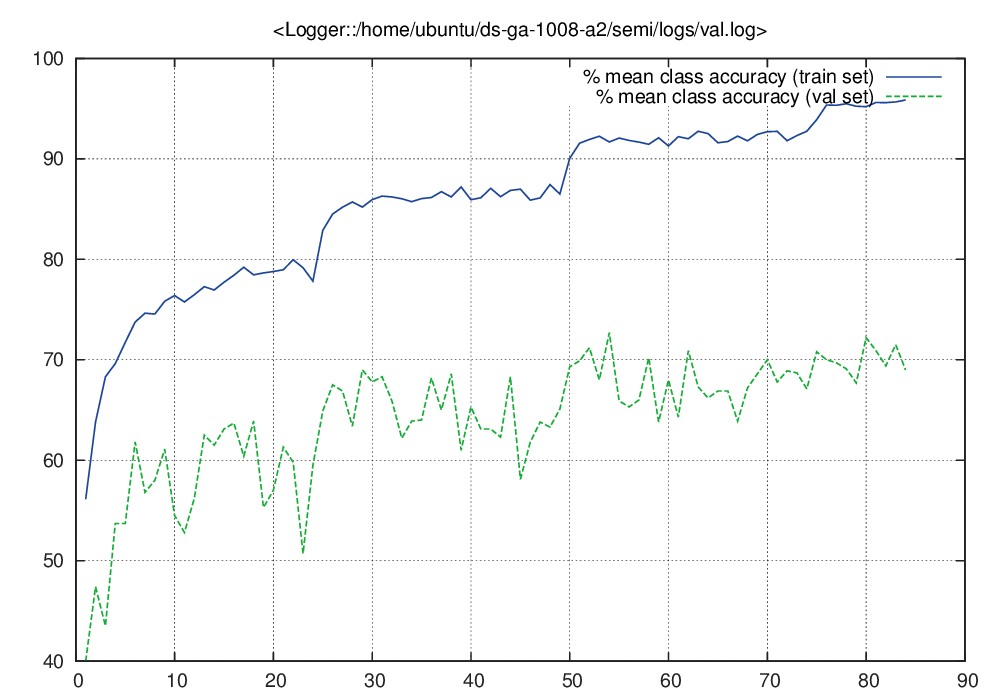
\includegraphics[width = 140mm, height=90mm]{../fig/pseudo_label/val_8800.png}
  \caption{Pseudo­labels training result: training set start from 7100 figures and end at 8800.}
\end{figure}

\subsection{Method: K­means Centroids + Pseudo­labels}


\\
\section{Visualization}
\subsection{Visualizing filters and augmentations}
Initially we were also trying to creat surrogate data set from 4000 unlabel figures, each figure will produced 100 surrogate figures and therefore we got 4000 class of 400000 figures in total. The initial figre is in the size of 3x96x96, and we created the surrogate figure by the size of 3x32x32 and each will subject in a random degree of rotation between -20 to 20, vertical and horizontal translate between 0 to 0.1, and scale in the range between 0.7 to 1.4. Figure 3.1 is the visualization of the surrogate figures.
\begin{figure}[H]
\centering
\begin{subfigure}
  \begin{tabular}{c}
  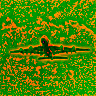
\includegraphics[width=50mm]{../fig/img_regNorm/2.png}
  \end{tabular}{}
\end{subfigure}
\begin{subfigure}
  \begin{tabular}{cccc}
  \subfloat{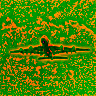
\includegraphics[width = 10mm]{../fig/img_regNorm/2.png}}&
  \subfloat{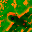
\includegraphics[width = 10mm]{../fig/img/2_1.png}}&
  \subfloat{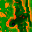
\includegraphics[width = 10mm]{../fig/img/2_2.png}}&
  \subfloat{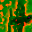
\includegraphics[width = 10mm]{../fig/img/2_19.png}}\\
  \subfloat{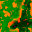
\includegraphics[width = 10mm]{../fig/img/2_3.png}}&
  \subfloat{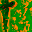
\includegraphics[width = 10mm]{../fig/img/2_4.png}}&
  \subfloat{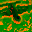
\includegraphics[width = 10mm]{../fig/img/2_5.png}}&
  \subfloat{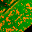
\includegraphics[width = 10mm]{../fig/img/2_10.png}}\\
  \subfloat{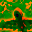
\includegraphics[width = 10mm]{../fig/img/2_25.png}}&
  \subfloat{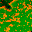
\includegraphics[width = 10mm]{../fig/img/2_26.png}}&
  \subfloat{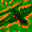
\includegraphics[width = 10mm]{../fig/img/2_29.png}}&
  \subfloat{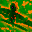
\includegraphics[width = 10mm]{../fig/img/2_30.png}}\\
  \subfloat{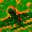
\includegraphics[width = 10mm]{../fig/img/2_32.png}}&
  \subfloat{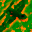
\includegraphics[width = 10mm]{../fig/img/2_33.png}}&
  \subfloat{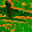
\includegraphics[width = 10mm]{../fig/img/2_34.png}}&
  \subfloat{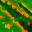
\includegraphics[width = 10mm]{../fig/img/2_35.png}}\\
  \subfloat{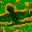
\includegraphics[width = 10mm]{../fig/img/2_37.png}}&
  \subfloat{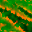
\includegraphics[width = 10mm]{../fig/img/2_38.png}}&
  \subfloat{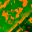
\includegraphics[width = 10mm]{../fig/img/2_41.png}}&
  \subfloat{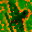
\includegraphics[width = 10mm]{../fig/img/2_48.png}}&
  \end{tabular}
\end{subfigure}
\caption{Figures of surrogate set}
\end{figure}
Then we implemented the kmeans method. According to the paper, they randomly extracted patches from unlabeled set of data, and performed kmean to find the centroids. The size of patch we extracted is 22x22 and we extracted 16 patches from total of 20000 unlabel figures. Number of centroids we obtained is 1600 because it produced good accuracy as the paper mentioned. As we can see from figure 3.2, most of the centroids are in very sharp of edge and color blobs.
\begin{figure}[H]
\centering
\begin{subfigure}
  \begin{tabular}{c}
  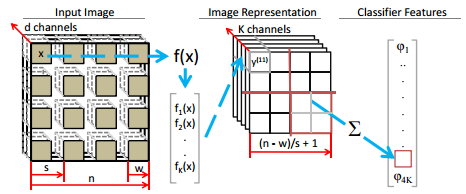
\includegraphics[width=100mm]{../fig/kmeansMethod.png}
  \end{tabular}{}
\end{subfigure}
\begin{subfigure}
  \begin{tabular}{cccc}
  \subfloat{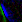
\includegraphics[width = 10mm]{../fig/center_20000_700/center4.png}}&
  \subfloat{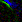
\includegraphics[width = 10mm]{../fig/center_20000_700/center5.png}}&
  \subfloat{
\includegraphics[width = 10mm]{../fig/center_20000_700/center6.png}}&
  \subfloat{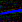
\includegraphics[width = 10mm]{../fig/center_20000_700/center8.png}}\\
  \subfloat{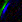
\includegraphics[width = 10mm]{../fig/center_20000_700/center12.png}}&
  \subfloat{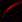
\includegraphics[width = 10mm]{../fig/center_20000_700/center22.png}}&
  \subfloat{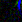
\includegraphics[width = 10mm]{../fig/center_20000_700/center23.png}}&
  \subfloat{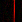
\includegraphics[width = 10mm]{../fig/center_20000_700/center24.png}}\\
  \subfloat{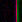
\includegraphics[width = 10mm]{../fig/center_20000_700/center28.png}}&
  \subfloat{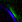
\includegraphics[width = 10mm]{../fig/center_20000_700/center30.png}}&
  \subfloat{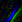
\includegraphics[width = 10mm]{../fig/center_20000_700/center36.png}}&
  \subfloat{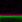
\includegraphics[width = 10mm]{../fig/center_20000_700/center37.png}}\\
  \subfloat{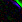
\includegraphics[width = 10mm]{../fig/center_20000_700/center38.png}}&
  \subfloat{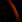
\includegraphics[width = 10mm]{../fig/center_20000_700/center41.png}}&
  \subfloat{
\includegraphics[width = 10mm]{../fig/center_20000_700/center46.png}}&
  \subfloat{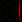
\includegraphics[width = 10mm]{../fig/center_20000_700/center49.png}}\\
  \subfloat{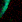
\includegraphics[width = 10mm]{../fig/center_20000_700/center50.png}}&
  \subfloat{
\includegraphics[width = 10mm]{../fig/center_20000_700/center52.png}}&
  \subfloat{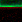
\includegraphics[width = 10mm]{../fig/center_20000_700/center57.png}}&
  \subfloat{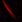
\includegraphics[width = 10mm]{../fig/center_20000_700/center58.png}}&
  \end{tabular}
\end{subfigure}
\caption{Figure of centroids}
\end{figure}

\subsection{t-SNE}
Here we took all the images from val.t7b, which contains 1000 figures for total and 100 figures in each of class. To generate t-SNE embedding, we used only the first channel of each of the image, which the dimension is 1x96x96, and feed it into manifold.embedding.tsne. Then we will get the mapping result for each of the image onto the 2D space, and we can plot the figures based on the mapped coordinate.

\begin{figure}[H]
\centering
\begin{subfigure}
  \begin{tabular}{cccc}
  \subfloat{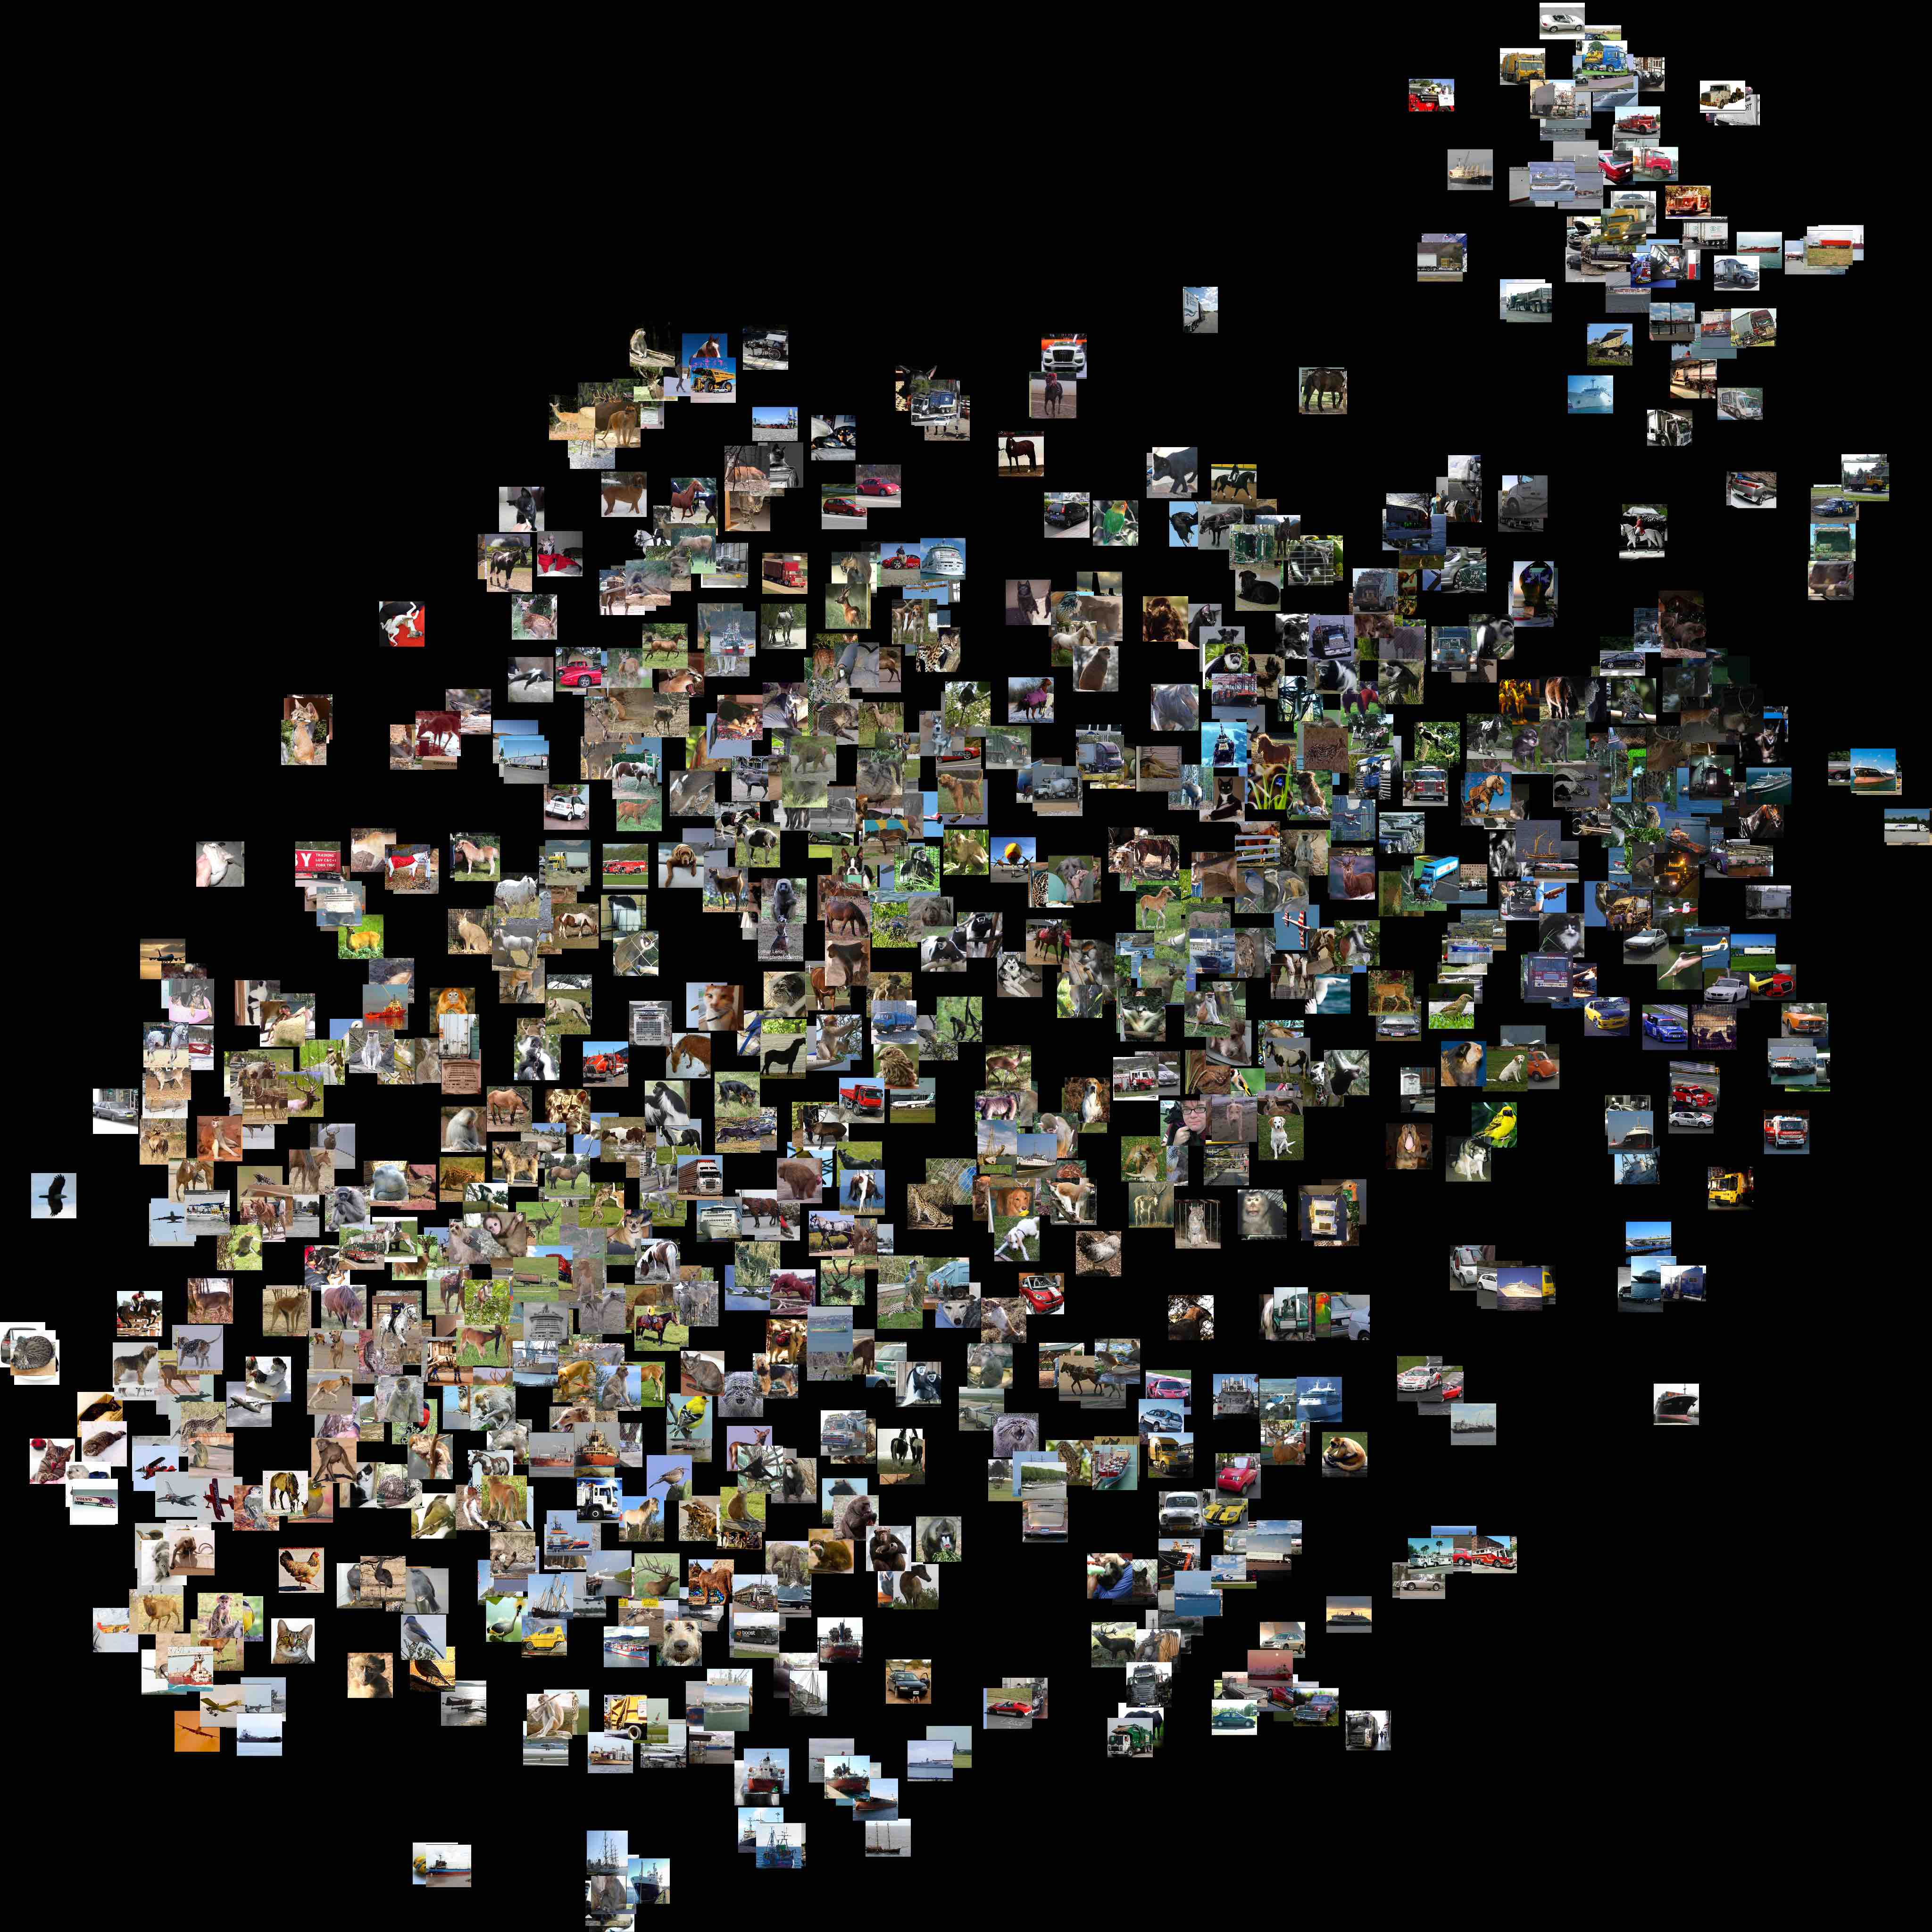
\includegraphics[width = 50mm]{../fig/t_SNEIII.jpeg}}&
  \subfloat{\includegraphics[width = 50mm]{../fig/t-SNE1_1.png}}&
  \subfloat{\includegraphics[width = 50mm]{../fig/t-SNE0_2.png}}\\
  \end{tabular}
\end{subfigure}
\caption{t-SNE Figure of original, layer before full-connected network, and layer after full-connected network}
\end{figure}

\end{document}

